\documentclass[12pt]{standalone}

\RequirePackage{times}
\RequirePackage{amsmath}
\RequirePackage{amssymb}
\RequirePackage[T1]{fontenc}

\usepackage{tikz}
\usepackage{xcolor}
\usepackage{pgfplots}
\pgfplotsset{compat=1.16}
\usetikzlibrary{arrows,backgrounds,scopes}

\definecolor{red}{HTML}{972e21}
\definecolor{yellow}{HTML}{ebb83f}
\definecolor{blue}{HTML}{5e7fbf}

\begin{document}
	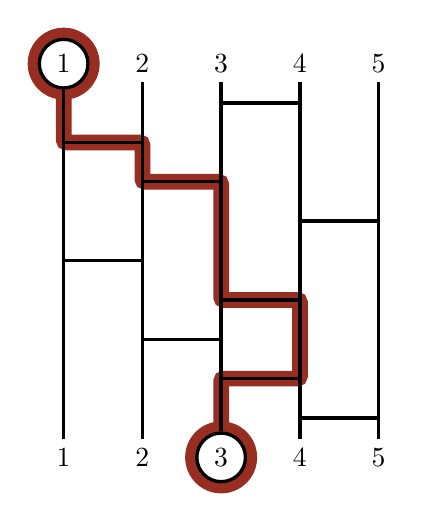
\begin{tikzpicture}
		\newcommand{\person}[2][]{\node[#1] (p#2) at (#2-1,0) {#2};}
		\newcommand{\goal}[2][]{\node[#1] (g#2) at (#2-1,-5) {#2};
			\draw[very thick] (p#2) -- (g#2);}
		
		\newcommand{\connection}[2]{\draw[very thick] (#1-1,#2*-0.5) -- (#1,#2*-0.5);}
		
		\person[circle,draw,very thick,fill=white]{1}
		\person{2}
		\person{3}
		\person{4}
		\person{5}
		
		\goal{1}
		\goal{2}
		\goal[circle,draw,very thick,fill=white]{3}
		\goal{4}
		\goal{5}
		
		\connection{3}{1}
		\connection{1}{2}
		\connection{2}{3}
		\connection{4}{4}
		\connection{1}{5}
		\connection{3}{6}
		\connection{2}{7}
		\connection{3}{8}
		\connection{4}{9}
		
		\begin{scope}[on background layer]
			\draw[fill, red] (p1) circle (0.45cm);
			\draw[fill, red] (g3) circle (0.45cm);
			\draw[red,line width=2mm,rounded corners=1pt] (p1) -- (0,-1) -- (1,-1) --(1,-1.5) -- (2, -1.5) -- (2, -3) -- (3, -3) -- (3, -4) -- (2, -4) -- (g3);
		\end{scope}
	\end{tikzpicture}
\end{document}